\documentclass[12pt, compress, aspectratio=1610]{beamer}

\usetheme{pl}

\usepackage{longtable}
\usepackage{booktabs}
\usepackage{minted}
\usepackage{listings}
\usepackage{color}
\usepackage{fancyvrb}
\newcommand{\VerbBar}{|}
\newcommand{\VERB}{\Verb[commandchars=\\\{\}]}
\DefineVerbatimEnvironment{Highlighting}{Verbatim}{commandchars=\\\{\},fontsize=\small}
% Add ',fontsize=\small' for more characters per line
\usepackage[framemethod=tikz]{mdframed}
\definecolor{shadecolor}{HTML}{EEEEEE}
\mdfsetup{
  backgroundcolor=shadecolor,
  linecolor=shadecolor,
  innerleftmargin=5pt,
  innerrightmargin=5pt,
  leftmargin=-5pt,
  rightmargin=-5pt,
  roundcorner=3pt
}
\newenvironment{Shaded}{\begin{mdframed}}{\end{mdframed}}
\newcommand{\KeywordTok}[1]{\textcolor[rgb]{0.26,0.66,0.93}{\textbf{{#1}}}}
\newcommand{\DataTypeTok}[1]{\textcolor[rgb]{0.74,0.68,0.62}{\underline{{#1}}}}
\newcommand{\DecValTok}[1]{\textcolor[HTML]{558B2F}{{#1}}}
\newcommand{\BaseNTok}[1]{\textcolor[HTML]{558B2F}{{#1}}}
\newcommand{\FloatTok}[1]{\textcolor[HTML]{558B2F}{{#1}}}
\newcommand{\ConstantTok}[1]{\textcolor[rgb]{0.74,0.68,0.62}{{#1}}}
\newcommand{\CharTok}[1]{\textcolor[HTML]{7E57C2}{{#1}}}
\newcommand{\SpecialCharTok}[1]{\textcolor[HTML]{7E57C2}{{#1}}}
\newcommand{\StringTok}[1]{\textcolor[HTML]{7E57C2}{{#1}}}
\newcommand{\VerbatimStringTok}[1]{\textcolor[HTML]{7E57C2}{{#1}}}
\newcommand{\SpecialStringTok}[1]{\textcolor[HTML]{7E57C2}{{#1}}}
\newcommand{\ImportTok}[1]{\textcolor[rgb]{0.74,0.68,0.62}{{#1}}}
\newcommand{\CommentTok}[1]{\textcolor[HTML]{546E7A}{\textit{{#1}}}}
\newcommand{\DocumentationTok}[1]{\textcolor[HTML]{BCAAA4}{\textit{{#1}}}}
\newcommand{\AnnotationTok}[1]{\textcolor[HTML]{BCAAA4}{\textbf{\textit{{#1}}}}}
\newcommand{\CommentVarTok}[1]{\textcolor[rgb]{0.74,0.68,0.62}{{#1}}}
\newcommand{\OtherTok}[1]{\textcolor[rgb]{0.74,0.68,0.62}{{#1}}}
\newcommand{\FunctionTok}[1]{\textcolor[HTML]{26A69A}{\textbf{{#1}}}}
\newcommand{\VariableTok}[1]{\textcolor[rgb]{0.74,0.68,0.62}{{#1}}}
\newcommand{\ControlFlowTok}[1]{\textcolor[rgb]{0.26,0.66,0.93}{\textbf{{#1}}}}
\newcommand{\OperatorTok}[1]{\textcolor[rgb]{0.74,0.68,0.62}{{#1}}}
\newcommand{\BuiltInTok}[1]{\textcolor[HTML]{42A5F5}{{#1}}}
\newcommand{\ExtensionTok}[1]{\textcolor[rgb]{0.74,0.68,0.62}{{#1}}}
\newcommand{\PreprocessorTok}[1]{\textcolor[rgb]{0.74,0.68,0.62}{\textbf{{#1}}}}
\newcommand{\AttributeTok}[1]{\textcolor[rgb]{0.74,0.68,0.62}{{#1}}}
\newcommand{\RegionMarkerTok}[1]{\textcolor[rgb]{0.74,0.68,0.62}{{#1}}}
\newcommand{\InformationTok}[1]{\textcolor[rgb]{0.00,0.40,1.00}{\textbf{\textit{{#1}}}}}
\newcommand{\WarningTok}[1]{\textcolor[HTML]{FF6E40}{\textbf{{#1}}}}
\newcommand{\AlertTok}[1]{\textcolor[HTML]{FF3D00}{{#1}}}
\newcommand{\ErrorTok}[1]{\textcolor[HTML]{DD2C00}{\textbf{{#1}}}}
\newcommand{\NormalTok}[1]{\textcolor[HTML]{212121}{{#1}}}

\makeatletter
\newsavebox\pandoc@box
\newcommand*\pandocbounded[1]{% scales image to fit in text height/width
  \sbox\pandoc@box{#1}%
  \Gscale@div\@tempa{\textheight}{\dimexpr\ht\pandoc@box+\dp\pandoc@box\relax}%
  \Gscale@div\@tempb{\linewidth}{\wd\pandoc@box}%
  \ifdim\@tempb\p@<\@tempa\p@\let\@tempa\@tempb\fi% select the smaller of both
  \ifdim\@tempa\p@<\p@\scalebox{\@tempa}{\usebox\pandoc@box}%
  \else\usebox{\pandoc@box}%
  \fi%
}
% Set default figure placement to htbp
\def\fps@figure{htbp}
\makeatother

\providecommand{\tightlist}{%
  \setlength{\itemsep}{0pt}\setlength{\parskip}{0pt}}

\let\OldTexttt\texttt
\renewcommand{\texttt}[1]{\OldTexttt{\color{codecolor}#1}}

\makeatletter
\def\maxwidth{\ifdim\Gin@nat@width>\linewidth\linewidth\else\Gin@nat@width\fi}
\makeatother

\newcommand{\begincols}{\begin{columns}}
\newcommand{\stopcols}{\end{columns}}
\newcommand{\roundpicture}[2]{%
\tikz\node[circle,
          text=white,
          minimum width=4cm,
          minimum height=4cm,
          path picture={
              \node at (path picture bounding box.center){
                  \includegraphics[width=4cm]{#1}
              };
          }]{#2};
}
\newcommand{\plain}[1]{%
\begin{picture}(0,0)
  \put(-28.5,-175){%
      \pgfuseimage{titlebackground}
  }
  \put(0,-145){%
      \begin{minipage}[b][4.5cm][t]{0.7\textwidth}
          \Large
          #1
      \end{minipage}
  }
\end{picture}
}

\title{Interpretable ML for biodiversity}
\subtitle{An introduction using species distribution models}
\date{\today}
\author{Timothée Poisot}
\institute{Université de Montréal}

\begin{document}

\maketitle

\begin{frame}{Main goals}
\phantomsection\label{main-goals}
\begin{enumerate}
\tightlist
\item
  How do we produce a model?
\item
  How do we convey that it works?
\item
  How do we talk about how it makes predictions?
\item
  How do we use it to guide actions?
\end{enumerate}
\end{frame}

\begin{frame}{The steps}
\phantomsection\label{the-steps}
\begin{enumerate}
\tightlist
\item
  Get data about species occurrences
\item
  Build a classifier and make it as good as we can
\item
  Measure its performance
\item
  Explain some predictions
\item
  Generate counterfactual explanations
\item
  Briefly discuss ensemble models
\end{enumerate}
\end{frame}

\begin{frame}{But why\ldots{}}
\phantomsection\label{but-why}
\begin{description}
\tightlist
\item[\ldots{} think of SDM as a ML problem?]
Because they are (and would be better if we accepted this)
\item[\ldots{} the focus on explainability?]
We cannot ask people to \emph{trust} - we must \emph{convince}
\end{description}
\end{frame}

\section{Introduction}\label{introduction}

\begin{frame}{Getting data}
\phantomsection\label{getting-data}
\end{frame}

\begin{frame}{Getting a polygon}
\phantomsection\label{getting-a-polygon}
\end{frame}

\begin{frame}{CHELSA2 data}
\phantomsection\label{chelsa2-data}
\end{frame}

\begin{frame}{Trimming polygon}
\phantomsection\label{trimming-polygon}
\end{frame}

\begin{frame}{Download data from GBIF}
\phantomsection\label{download-data-from-gbif}
\end{frame}

\section{Validation}\label{validation}

\begin{frame}[fragile]{Pseudo-absences}
\phantomsection\label{pseudo-absences}
\begin{verbatim}
SDM Layer with 45336 Bool cells
    Proj string: +proj=longlat +datum=WGS84 +no_defs
    Grid size: (239, 543)
\end{verbatim}
\end{frame}

\begin{frame}{Visu}
\phantomsection\label{visu}
\pandocbounded{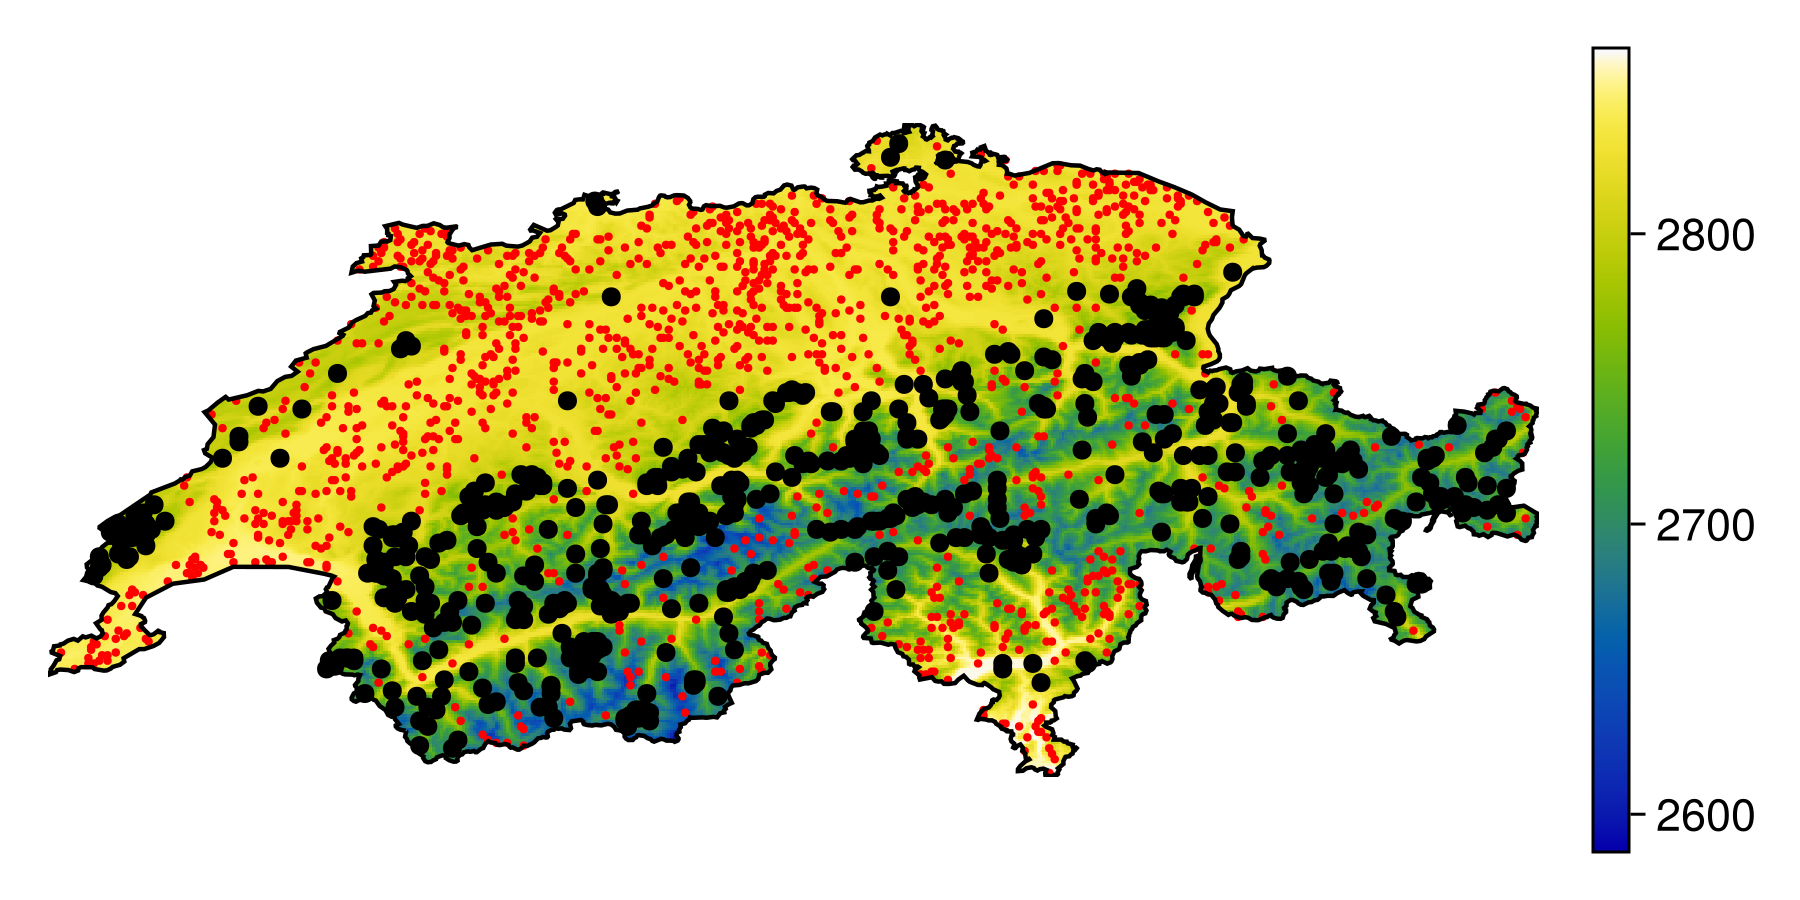
\includegraphics[keepaspectratio]{figures/slides_8_1.png}}~
\end{frame}

\section{Model setup}\label{model-setup}

\begin{frame}[fragile]{Setup}
\phantomsection\label{setup}
\begin{verbatim}
SDeMo.MultivariateTransform{MultivariateStats.PCA} → SDeMo.NaiveBayes → P(x
) ≥ 0.5
\end{verbatim}
\end{frame}

\begin{frame}[fragile]{Cross-validation}
\phantomsection\label{cross-validation}
\begin{verbatim}
0.5620979518435002
\end{verbatim}
\end{frame}

\begin{frame}[fragile]{re-training}
\phantomsection\label{re-training}
\begin{verbatim}
SDeMo.MultivariateTransform{MultivariateStats.PCA} → SDeMo.NaiveBayes → P(x
) ≥ 0.281
\end{verbatim}
\end{frame}

\begin{frame}[fragile]{Initial pred}
\phantomsection\label{initial-pred}
\begin{verbatim}
SDM Layer with 69967 Float64 cells
    Proj string: +proj=longlat +datum=WGS84 +no_defs
    Grid size: (239, 543)
\end{verbatim}
\end{frame}

\begin{frame}{Visu}
\phantomsection\label{visu-1}
\pandocbounded{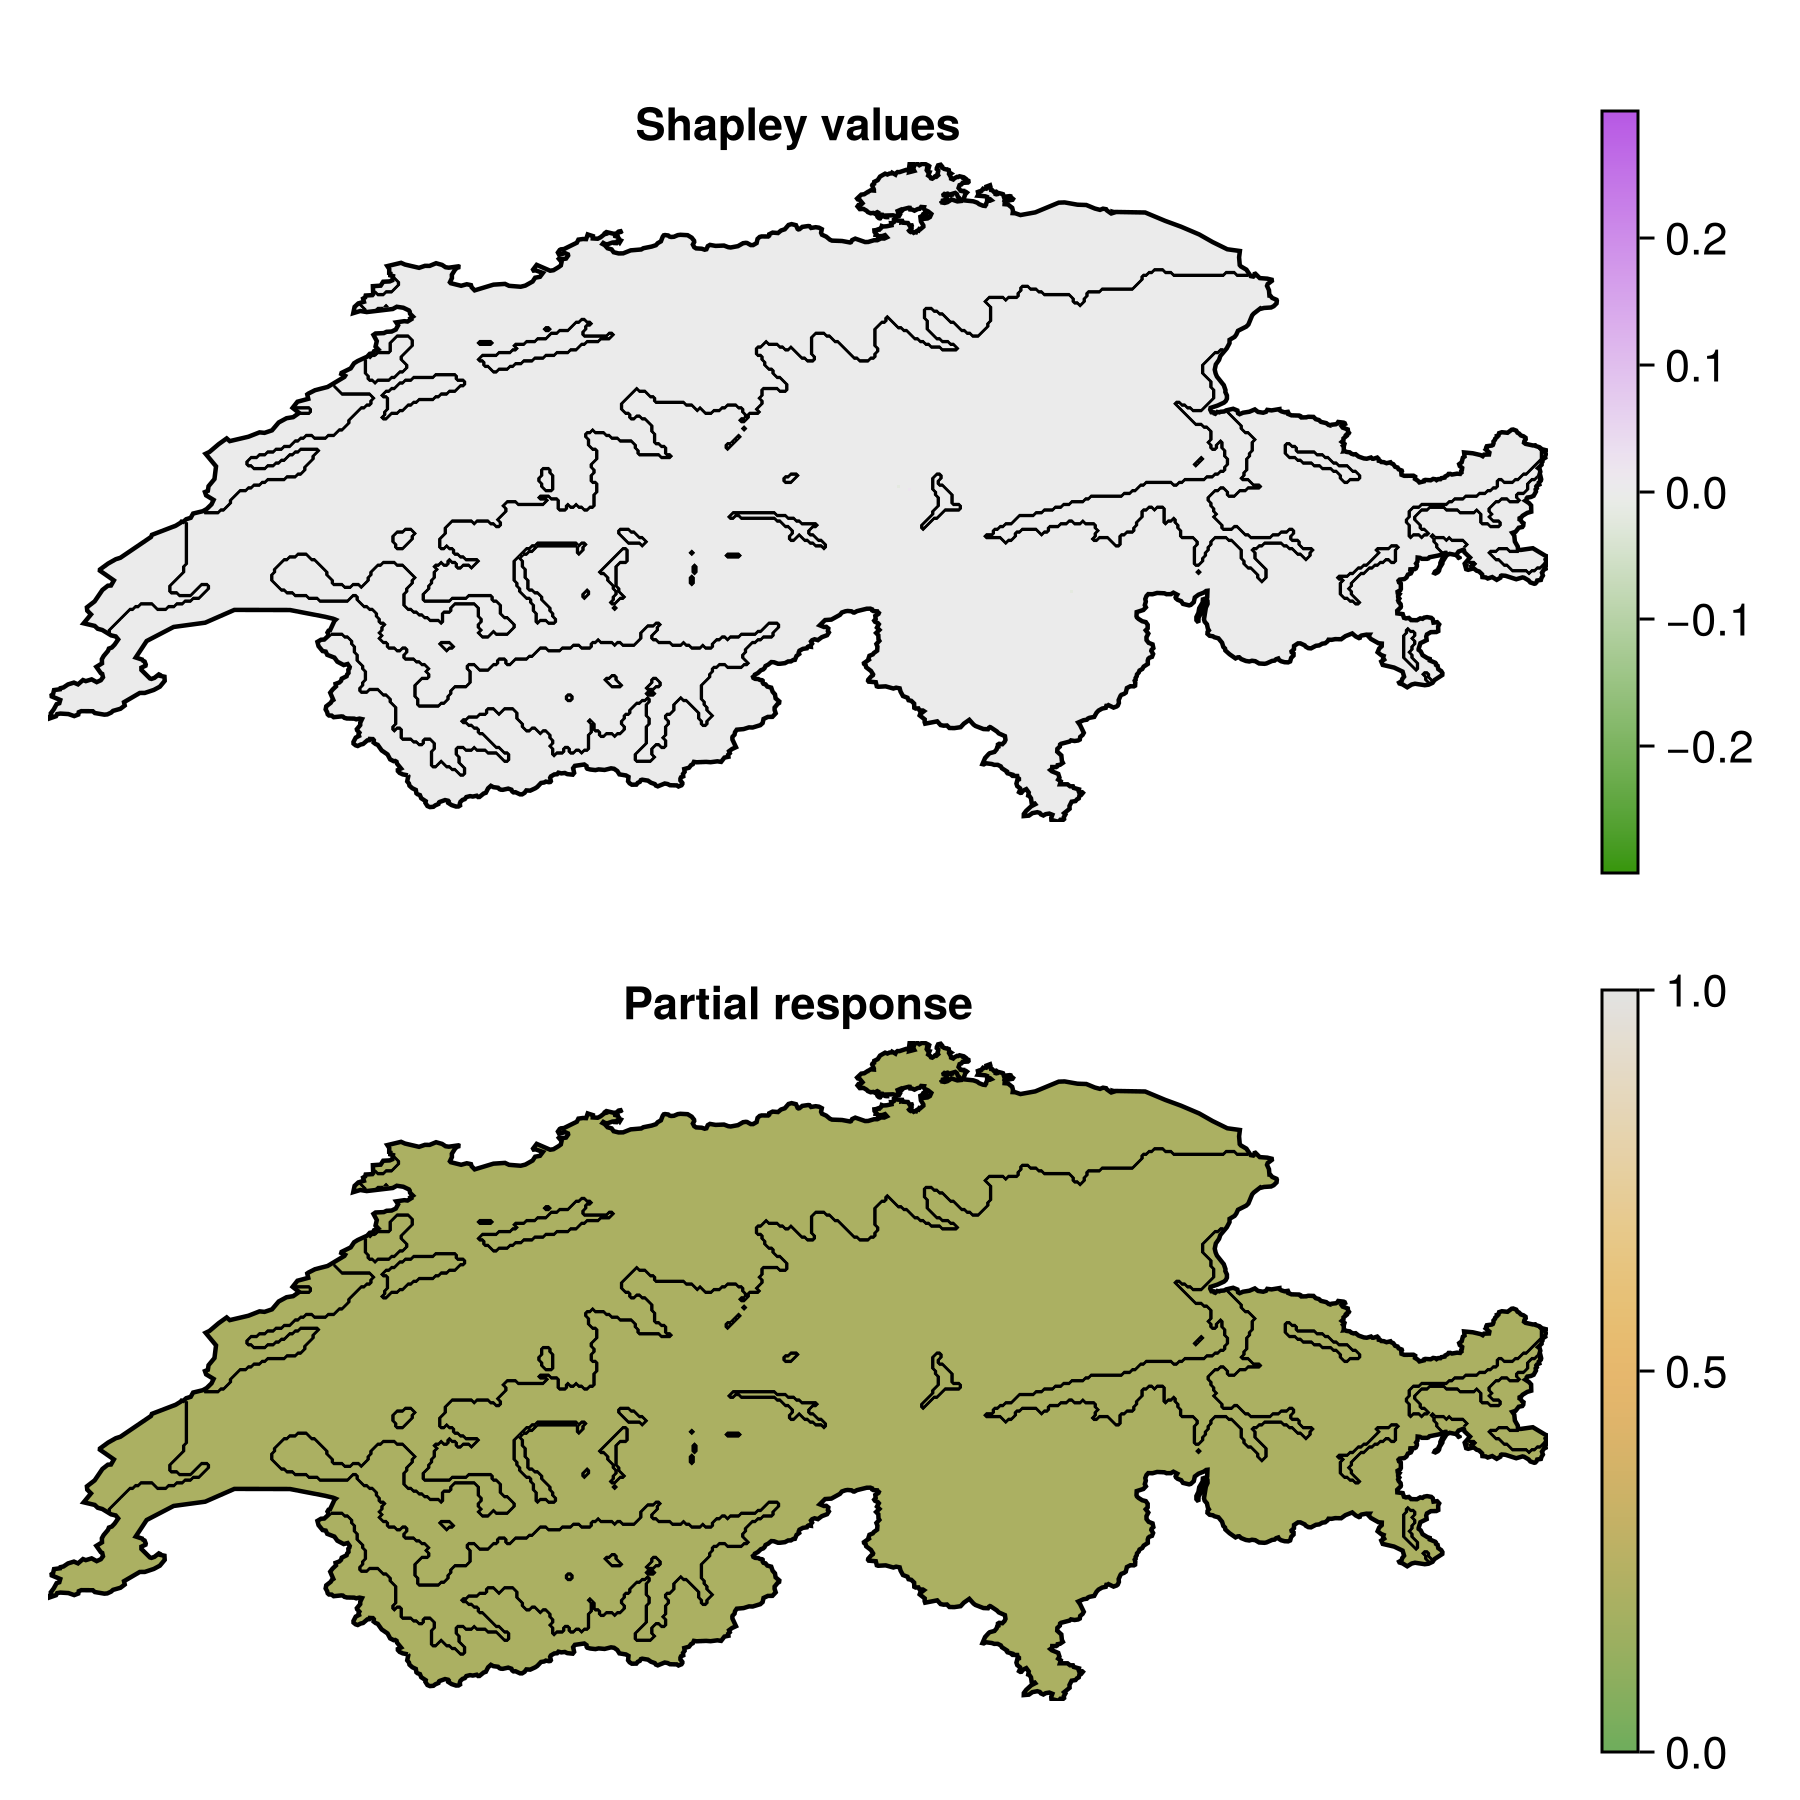
\includegraphics[keepaspectratio]{figures/slides_13_1.png}}~
\end{frame}

\section{Why?}\label{why}

\begin{frame}{code}
\phantomsection\label{code}
\end{frame}

\begin{frame}{Visu}
\phantomsection\label{visu-2}
\pandocbounded{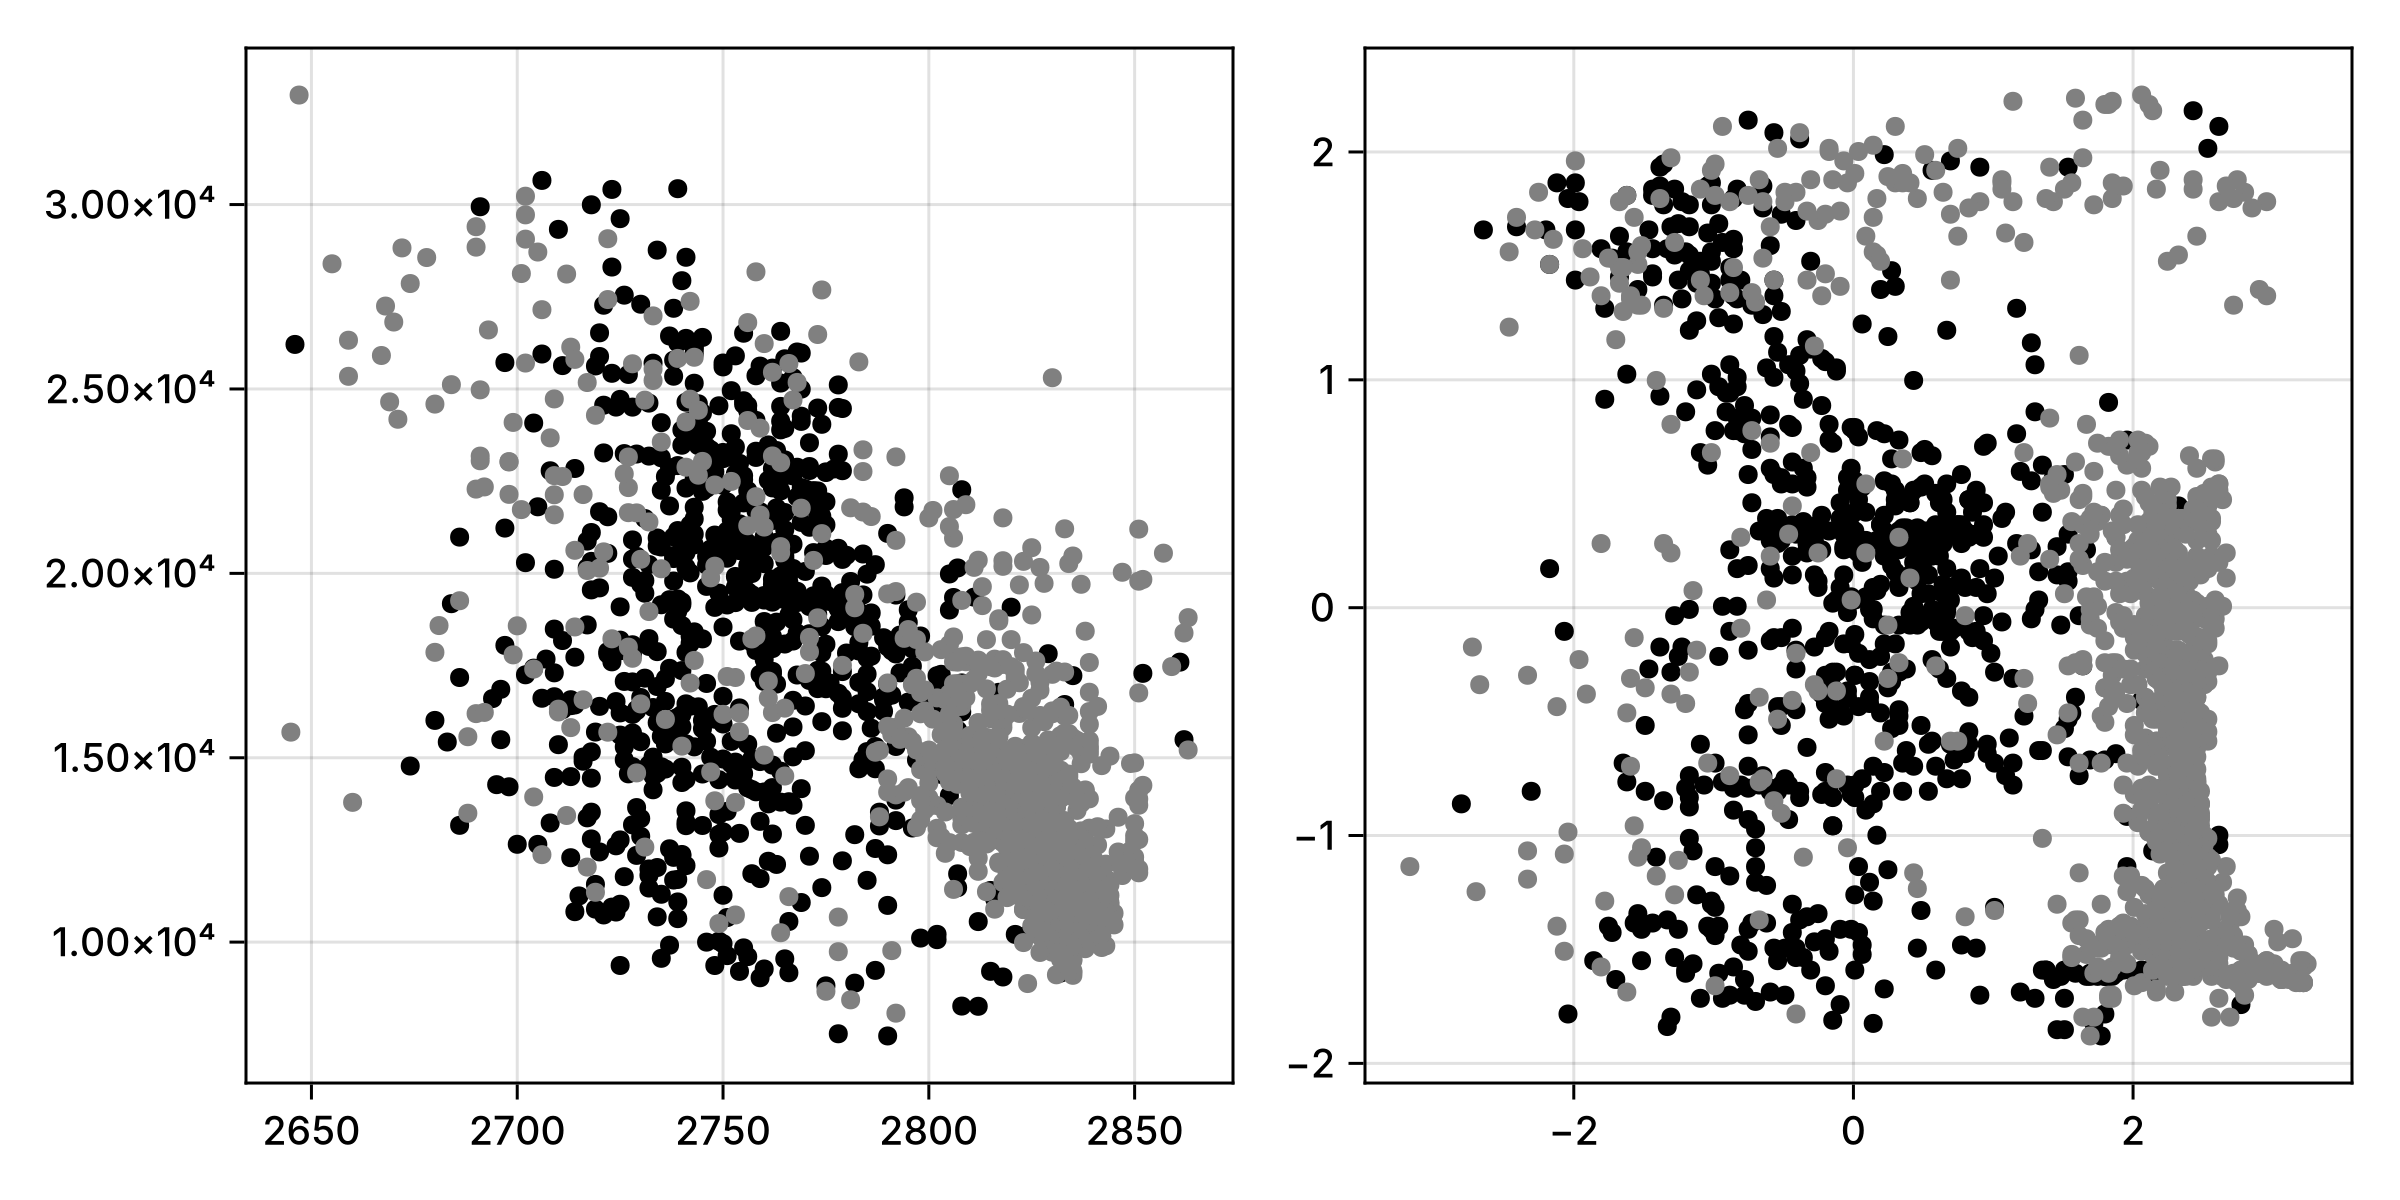
\includegraphics[keepaspectratio]{figures/slides_15_1.png}}~
\end{frame}

\begin{frame}[fragile]{mosaic}
\phantomsection\label{mosaic}
\begin{verbatim}
SDM Layer with 69967 Int64 cells
    Proj string: +proj=longlat +datum=WGS84 +no_defs
    Grid size: (239, 543)
\end{verbatim}
\end{frame}

\begin{frame}{visu}
\phantomsection\label{visu-3}
\pandocbounded{
\includegraphics[keepaspectratio]{figures/slides_17_1.png}}~
\end{frame}

\section{About ensemble models}\label{about-ensemble-models}

\begin{frame}[fragile]{Uncertainty}
\phantomsection\label{uncertainty}
\begin{verbatim}
0.6537641876644507
\end{verbatim}
\end{frame}

\begin{frame}[fragile]{Add pred}
\phantomsection\label{add-pred}
\begin{verbatim}
SDM Layer with 69967 Float64 cells
    Proj string: +proj=longlat +datum=WGS84 +no_defs
    Grid size: (239, 543)
\end{verbatim}
\end{frame}

\begin{frame}{Visu 2}
\phantomsection\label{visu-2-1}
\pandocbounded{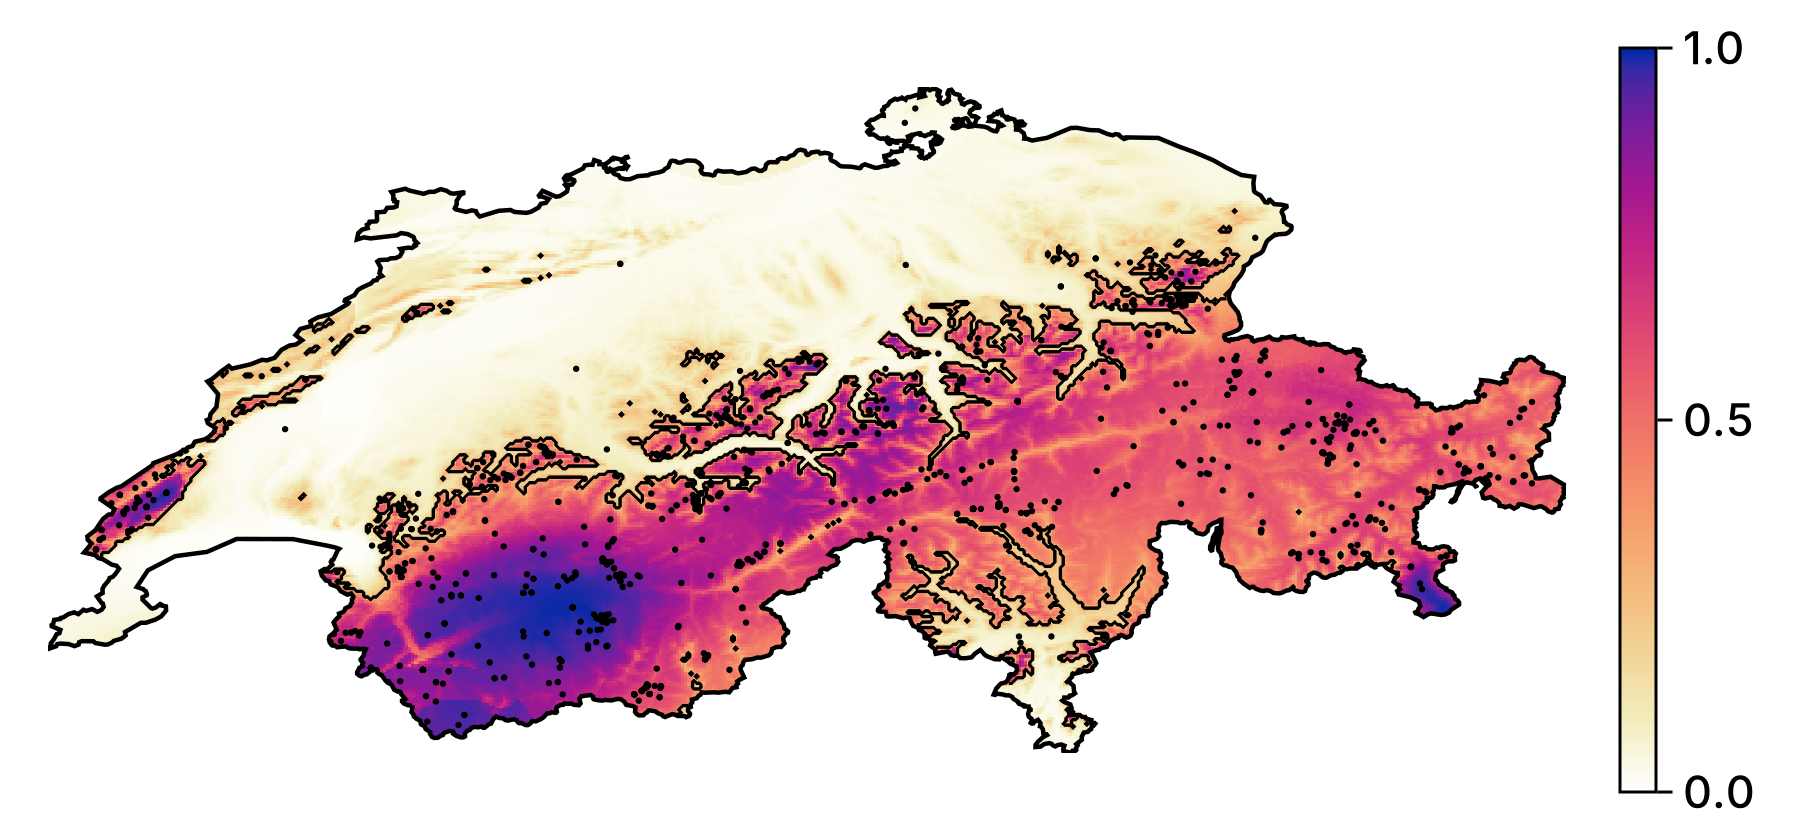
\includegraphics[keepaspectratio]{figures/slides_20_1.png}}~
\end{frame}

\begin{frame}[plain]
  \begin{picture}(0,0)
    \put(-28.5,-175){%
      \pgfuseimage{titlebackground}
    }
  \end{picture}
\end{frame}

\end{document}
